\chapter{Communication With openHAB}
\label{appendix:communication-with-openhab}

The open source home automation hub openHAB described in \Cref{sec:analysis:choice-of-hub} exposes an API with a REST architecture. Clients can communicate with the API over HTTP.

The communication with the openHAB API consists of the following two components.

\begin{description}
\item[REST client] A base REST client suitable for communicating with a REST API which carries its data using JSON. The client implements base methods for interacting with a REST API. This includes retrieving, deleting, updating and creating entities. The base client parses data received by the API into models.
\item[openHAB client] The client builds on top of the base REST client and adds openHAB specific methods. This includes retrieving things and items as well as updating the state of an item.
\end{description}

\Cref{fig:communication-with-openhab:class-diagram-rest-client} shows a class diagram of the REST client. The involved components are briefly described below.

\begin{description}
\item[RESTClient] The base REST client which is responsible for performing requests and mapping response to models that can be further processed or displayed in the application.
\item[RequestQueue] Responsible for creating worker threads for network requests.
\item[ResultListener] Interface implemented by objects that should receive a result when a network request completes, either because of a failure or because of a successful response.
\item[EntityBuilder] Interface implemented by objects mapping from the received JSON to models.
\item[Result] Encapsulates a network result. A result can either be a success or a failure. In case of a success, the result will contain a the value received from the API. In case of a failure, the result must contain an error.
\end{description}

\begin{figure}[h!]
\centering
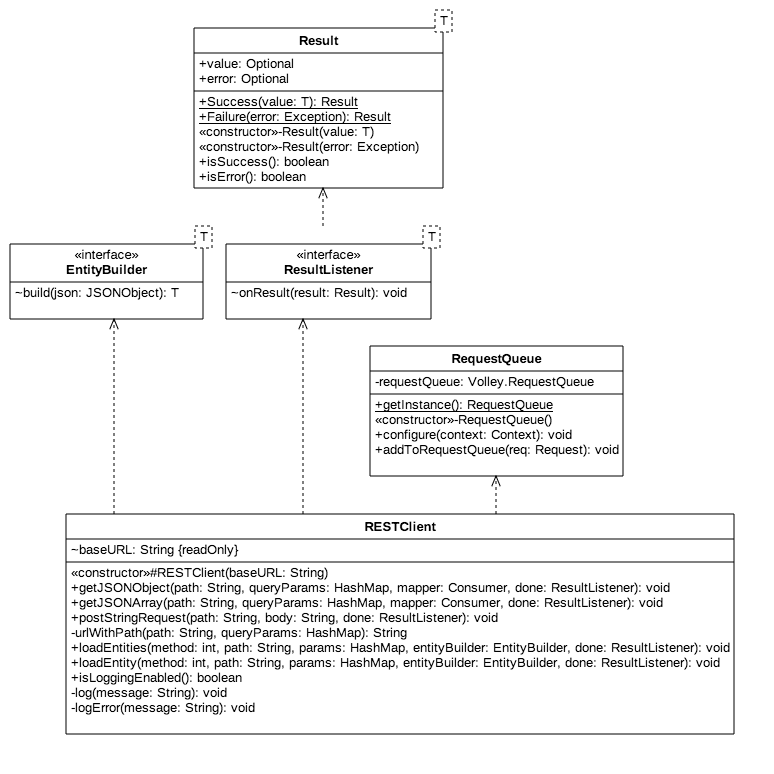
\includegraphics[width=\textwidth]{images/uml-rest-client}
\caption{Class diagram showing the architecture of the REST client used for communicating with a REST API.}
\label{fig:communication-with-openhab:class-diagram-rest-client}
\end{figure}

\Cref{fig:communication-with-openhab:class-diagram-openhab-client} shows a class diagram of the openHAB client. The involved components are briefly described below.

\begin{description}
\item[OpenHABClient] A specialisation of the base REST client implementing openHAB specific functionality.
\item[BooleanResult] Similar to the Result, this either represents a success or a failure. In the case of a success, the BooleanResult does not contain a value.
\item[Item] Model representing an item in openHAB.
\item[Thing] Model representing a thing in openHAB.
\end{description}

\begin{figure}[h!]
\centering
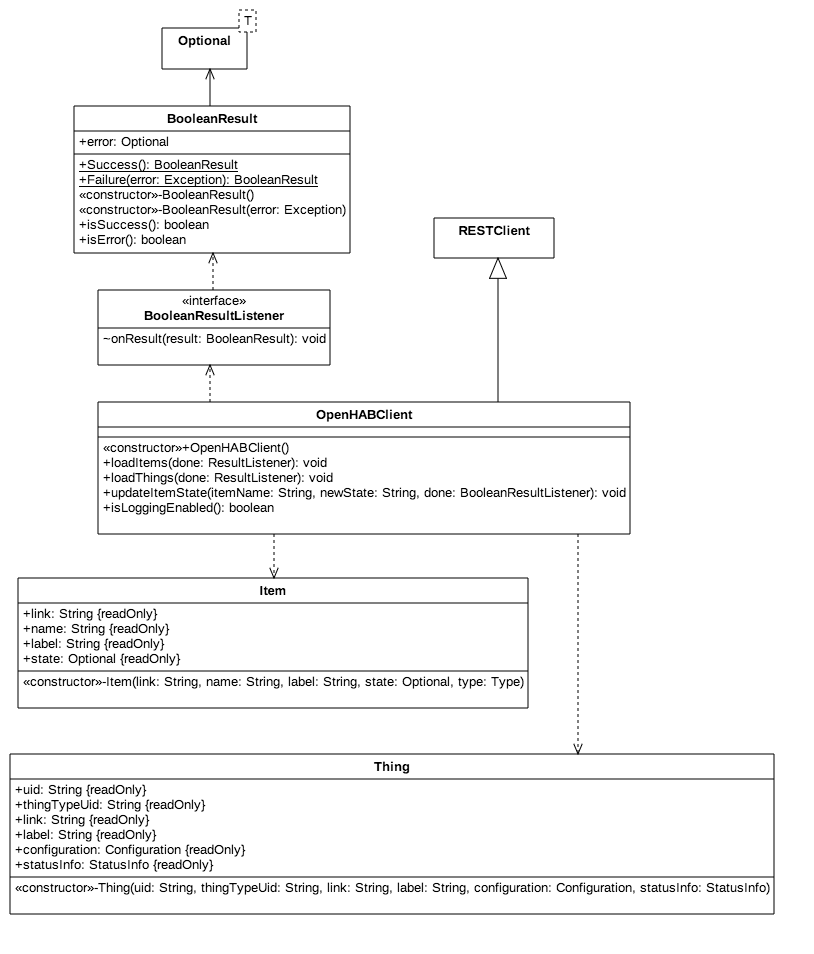
\includegraphics[width=\textwidth]{images/uml-openhab-client}
\caption{Class diagram showing the architecture of the openHAB client used for communicating with the openHAB API}
\label{fig:communication-with-openhab:class-diagram-openhab-client}
\end{figure}

%%% Local Variables:
%%% mode: latex
%%% TeX-master: "../master"
%%% End:
